\documentclass{standalone}
\usepackage{tikz}
\begin{document}
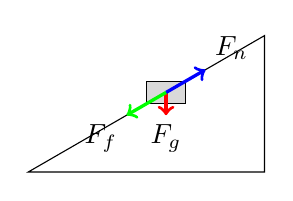
\begin{tikzpicture}
    % Define the angle for inclination
    \def\angle{30}
    % Draw the inclined plane
    \draw (0, 0) -- (3, 0) -- (3,{3*tan(\angle)}) -- cycle;
    % Draw the block
    \draw[fill=gray!30] (1.5, {1.5*tan(\angle)}) rectangle (2, {2*tan(\angle)});
    % Draw the forces
    % Gravitational force
    \draw[very thick, ->, red]  (1.75, {1.75*tan(\angle)}) --  (1.75, {1.25*tan(\angle)});
    \node[below] at (1.75, {1.25*tan(\angle)}) {$F_g$};
    % Normal force
    \draw[very thick, ->, blue] (1.75, {1.75*tan(\angle)}) --  (2.25, {2.25*tan(\angle)});
    \node[above right] at (2.25, {2.25*tan(\angle)}) {$F_n$};
    % Frictional force
    \draw[very thick, ->, green]  (1.75, {1.75*tan(\angle)}) -- (1.25, {1.25*tan(\angle)});
    \node[below left] at (1.25, {1.25*tan(\angle)}) {$F_f$};
\end{tikzpicture}
\end{document}